\chapter{Results and Comparisons}
\label{chap:results}

% This chapter presents the experimental results obtained from the methods listed in the previous section.

This section presents the experimental results corresponding to the three primary objectives outlined in Chapter~\ref{chap:methods}. Specifically, Section~\ref{sec:results_fpga} discusses the outcomes and performance improvements observed when deploying trained DiffLogic models onto FPGA hardware. Section~\ref{sec:results_compression} evaluates the effectiveness of the MiniNet compression algorithm in reducing network complexity without compromising accuracy. Finally, Section~\ref{sec:results_visualization} describes the development and initial results obtained from two novel visualization tools aimed at enhancing model interpretability.

\section{Results from Deploying Learned Logic on Hardware}
\label{sec:results_fpga}



%% !! CAN ADD THE FOLLOWING PARTS ON THE METHODS SECTION, BUT MIGHT BE TOO MUCH
% A key question is how an FPGA implementation of DiffLogic compares to inference on a conventional GPU. Although GPUs are highly optimized for massive parallel arithmetic, they are less specialized for arbitrary logic. Since DiffLogic inference on a CPU already operates efficiently at the bit level, the benefit of mapping to an FPGA is not guaranteed. Nonetheless, four dimensions inform this comparison:

% \begin{itemize}[noitemsep,topsep=0pt]
%     \item \textbf{Latency:} On an FPGA, latency depends on signal propagation through logic (tens of nanoseconds). On a GPU, overheads include kernel launch and possible memory transfers.
%     \item \textbf{Throughput:} An FPGA clocked at 50\,MHz can achieve up to
%     50~million inferences per second when fully pipelined. GPUs, however, can also process millions of inferences in parallel batches.
%     \item \textbf{Parallelism:} An FPGA can instantiate multiple copies of the circuit (as resources allow), whereas a GPU leverages SIMD data parallelism.
%     \item \textbf{Energy Efficiency:} FPGAs are generally more power-efficient for fixed logic operations, especially if the GPU is underutilized.
% \end{itemize}

An important question addressed is how FPGA implementations of DiffLogic compare to traditional GPU-based inference, as DiffLogic models are inherently composed of logic gates, making FPGA implementations suitable as they are optimized for logic operations. GPUs, while highly optimized for arithmetic parallelism, tend to be less efficient with arbitrary logic typical in DiffLogic models. Given the already efficient bit-level CPU implementation of DiffLogic, it was important to empirically assess whether mapping these logic-gate-based models onto an FPGA would yield meaningful performance gains.

Twenty-five trained DiffLogic models with varying node counts were evaluated to measure inference scalability. Two deployment modes were tested:
(i) GPU-based DiffLogic inference,
(ii) FPGA-based Boolean circuit synthesis.


\begin{figure}[htbp]
    \centering
    \begin{subfigure}[b]{0.48\textwidth}
        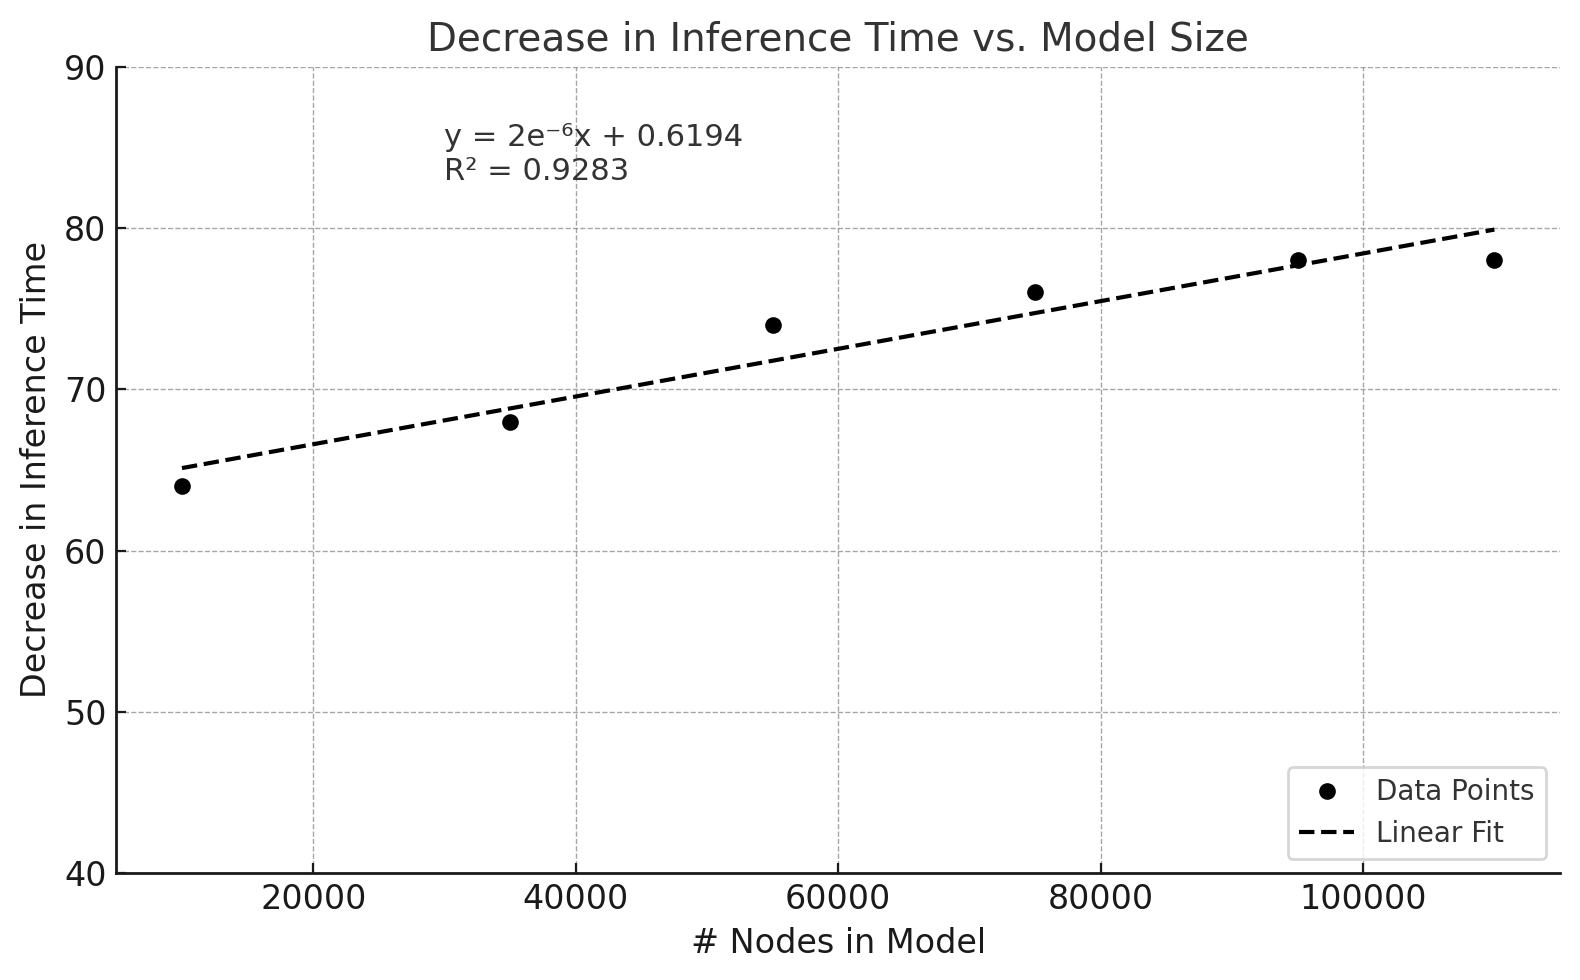
\includegraphics[width=\linewidth]{Figures/fpga-graph-1.png}
        \caption{Decrease in inference time vs. number of nodes.}
        \label{fig:graph1}
    \end{subfigure}
    \hfill
    \begin{subfigure}[b]{0.48\textwidth}
        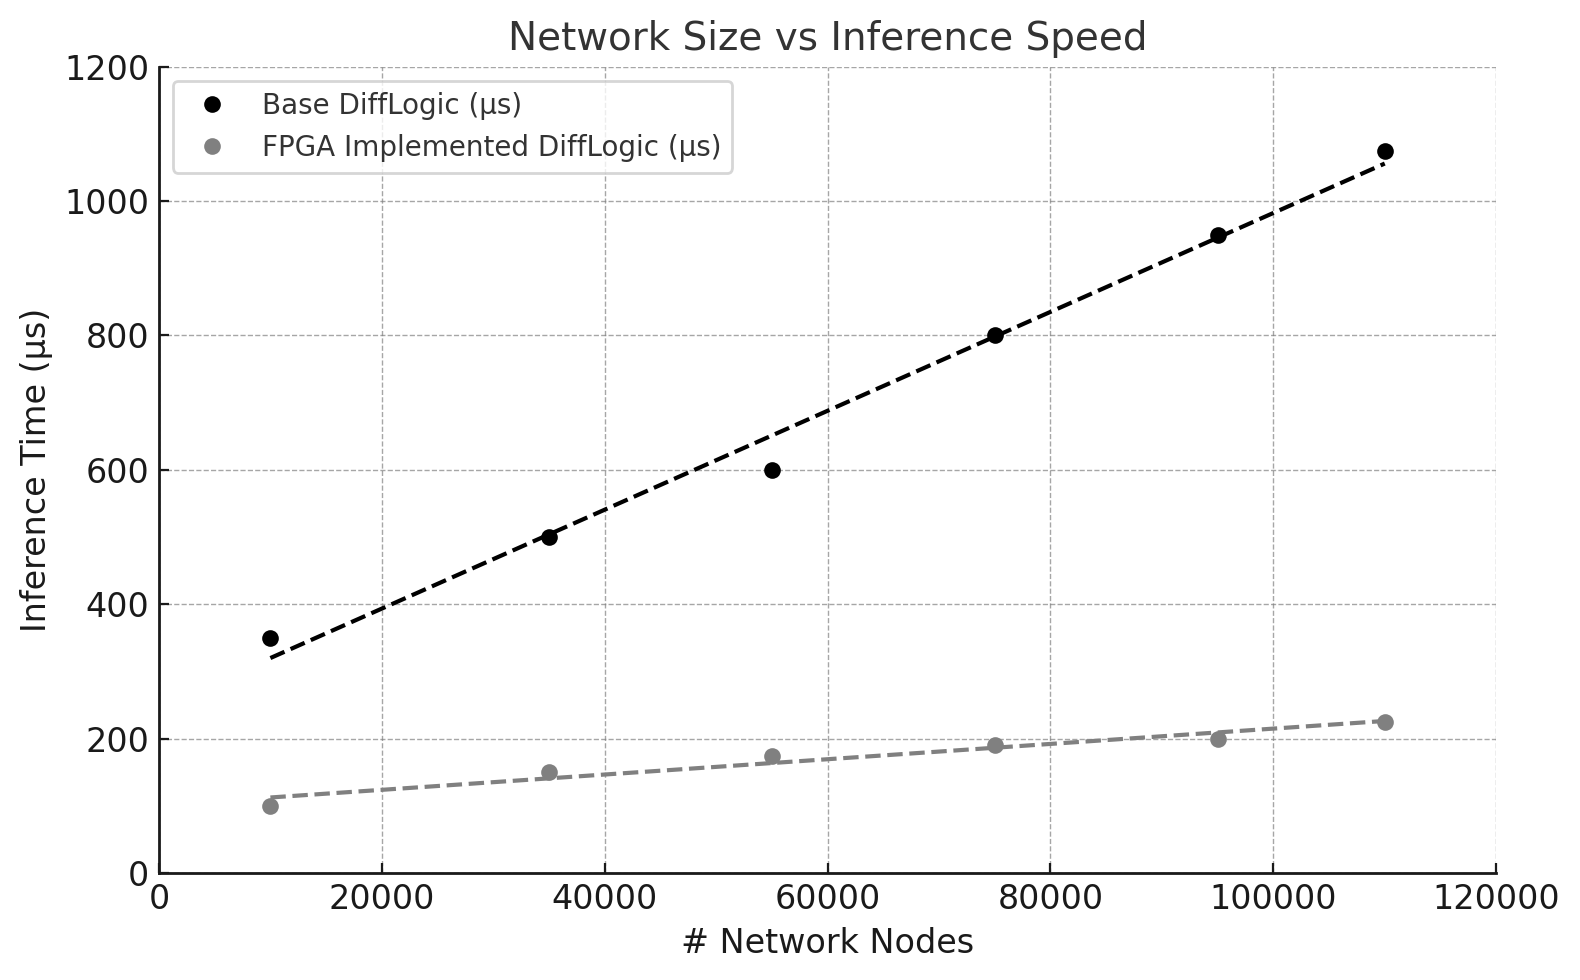
\includegraphics[width=\linewidth]{Figures/fpga-graph-2.png}
        \caption{Inference time between GPU and FPGA}
        \label{fig:graph2}
    \end{subfigure}
    \caption{Comparison of model inference improvements.}
    \label{fig:fpga_comparison}
\end{figure}


Table~\ref{tab:fpga_comparison} compares inference times, highlighting significant FPGA speedups. As network sizes grow, FPGA implementations increasingly outperform GPUs, achieving up to 78\% reductions in inference time for the largest models tested. Figure~\ref{fig:graph1} (left) illustrates this relationship, demonstrating a strong correlation ($R^2=0.9283$) that suggests FPGA advantages grow with network size. The right panel of Figure~\ref{fig:graph2} (right) further emphasizes FPGA latency improvements over GPU implementations. Additionally, it is noted that the largest tested network occupied only about 13\% of available LUTs, thus permitting additional logic or multiple circuit instances.

\begin{table}[htbp]
\caption{Inference Time: GPU-Based vs. FPGA-Based DiffLogic Networks}
\label{tab:fpga_comparison}
\begin{tabularx}{\textwidth}{lXXX}
\hline
Nodes & DiffLogic ($\mu$s) & FPGA ($\mu$s) & \% Decrease \\
\hline
51,200   & 365.7   & 139.46 & 62\% \\
614,400  & 724.28  & 280.52 & 74\% \\
819,200  & 907.78  & 202.54 & 78\% \\
1,108,160 & 1086.52 & 239.64 & 78\% \\
\hline
\end{tabularx}
\end{table}


Given that DiffLogic on GPUs already significantly outperforms standard deep neural networks~\cite{difflogic}, the observed FPGA speedups are especially notable. Future research will further explore scalability beyond one million nodes, examine energy consumption, memory efficiency, and investigate pipeline optimization strategies. Overall, FPGA deployment of DiffLogic offers substantial improvements in inference latency, particularly valuable for real-time and resource-constrained applications.


% The DE10-Lite board allows mapping of inputs (such as DIP switches or GPIO pins) to the circuit’s input ports and uses on-board LEDs or external interfaces for outputs. In one demonstration, an emulated RAM was controlled via DIP switches to provide a pre-loaded image’s bits as inputs. For more exhaustive validation, the generated Verilog code can be testbenched in ModelSim, supplying synthetic input frames and examining intermediary signals for debugging purposes.

% \textbf{FPGA Synthesis, Timing, and Deployment}

% Synthesis is conducted using Intel’s Quartus Prime software to confirm that the purely combinational circuit (unless registers are added for pipelining) fits within the DE10-Lite’s 22{,}320 logic elements. Typical DiffLogic networks require a few hundred to a few thousand two-input LUTs, remaining well within capacity. A 50\,MHz timing constraint was introduced to ensure the combinational path (up to about ten logic levels) meets a 20\,ns propagation requirement, which was met successfully.

% Following synthesis, the bitstream is programmed onto the DE10-Lite, transforming the FPGA into a hardware embodiment of the learned model. Each inference is then a direct propagation of signals through these gates, effectively bypassing the need for multipliers or large memory blocks common in other neural network FPGA designs. Quartus reports indicate that even the largest tested network occupies only about 13\% of the LUTs with minimal routing congestion, leaving headroom for additional instances or other logic.

% Although clocking is not strictly necessary for pure combinational logic, the DE10-Lite’s design requires a clock when interfacing with on-board RAM or other peripherals, limiting input switching to around 50\,MHz in practice. This constraint did not pose a problem for manually controlled inputs, and preliminary indications suggest that power consumption for a small combinational network on FPGA is substantially lower than GPU-based inference, reinforcing the suitability of this approach for low-power or edge-centric scenarios.





\section{Results from Compressing Trained DiffLogic Networks}
\label{sec:results_compression}

Although FPGA implementations of DiffLogic provide fast inference, the full, uncompressed models (``parent models'') are large and contain many rarely activated gates. To improve efficiency, the MiniNet compression algorithm (Section \ref{sec:mininets}) prunes these infrequently used gates, maintaining essential decision-making structures. This yields models that are computationally simpler, faster, and more interpretable.

To evaluate MiniNet performance, five DiffLogic models with varying layers and nodes were trained until surpassing 90\% accuracy on a binarized MNIST dataset (cropped to 20x20 pixels, 80-20 train-test split, learning rate of 0.01, grad factor = 1, temperature parameter $\tau=10$). The selected network had two layers of 2500 nodes each, reaching 91.2\% accuracy. While larger DiffLogic models achieve state-of-the-art performance \cite{difflogic}, this research prioritizes interpretability through smaller models. Future work aims to assess MiniNet performance on larger networks.

\begin{table}[htbp]
\caption{MiniNet Performance Compared to the Parent DiffLogic Network with 5010 gates}
\label{tab:mininets}
\begin{tabularx}{\textwidth}{lXXXXXXX}
\hline
Class & \% Time Red & \% Size Red & Accuracy & Precision & Recall & F1 \\
\hline
Class 0 & -9.8\% & -85.5\% & 97.2\% & 79.2\% & 11.1\% & 0.87 \\
Class 1 & -10.0\% & -85.6\% & 98.6\% & 89.5\% & 10.9\% & 0.93 \\
Class 2 & -10.1\% & -85.5\% & 94.2\% & 64.7\% & 10.9\% & 0.76 \\
Class 3 & -10.2\% & -85.5\% & 94.0\% & 63.5\% & 11.2\% & 0.76 \\
Class 4 & -10.1\% & -85.6\% & 95.0\% & 68.2\% & 11.0\% & 0.79 \\
Class 5 & -10.1\% & -85.5\% & 93.4\% & 61.5\% & 10.8\% & 0.74 \\
Class 6 & -10.1\% & -85.5\% & 96.7\% & 76.6\% & 11.1\% & 0.85 \\
Class 7 & -10.1\% & -85.5\% & 96.1\% & 74.0\% & 10.7\% & 0.83 \\
Class 8 & -10.2\% & -85.5\% & 90.4\% & 51.2\% & 10.9\% & 0.65 \\
Class 9 & -10.3\% & -85.5\% & 91.9\% & 55.8\% & 11.1\% & 0.70 \\
Average & -10.0\% & -86.0\% & 94.8\% & 68.4\% & 11.0\% & 0.79 \\
$\pm$ Std. & $\pm$0.1\% & $\pm$0.1\% & $\pm$2.5\% & $\pm$11.5\% & $\pm$0.1\% & $\pm$0.085 \\
\hline
\end{tabularx}
\end{table}


Initial tests with a DiffLogic model containing 5010 gates (two layers of 2500 gates and 10 output nodes) shown in Table~\ref{tab:mininets} demonstrated that MiniNets achieved class-score inference in 337$\mu$s on average and a one-versus-all accuracy of 94.8\%. Notably, this accuracy surpassed the parent model’s due to increased true negatives per class.

Additionally, MiniNet compression significantly reduces model complexity, achieving approximately 86\% reduction in size and a 10\% average reduction in inference time. Consequently, only around 14\% of the original gates are needed per class-specific prediction, facilitating faster inference.



% However, these efficiency gains a modest trade-off, with MiniNet accuracy dropping by approximately 3.8% compared to the parent model. Nonetheless, reduced computational demands and improved interpretability justify this compromise, particularly in resource-constrained or interpretability-critical scenarios.

% Overall, MiniNet effectively eliminates extraneous logic gates, substantially reducing model complexity and inference times. The slight accuracy decline is acceptable, given the substantial gains in efficiency and interpretability.







% maybe run some experiments on different thresholds. I remember we used different approaches towards creating MiniNets, as the one I used was based on counting the Switching Probability for a specific gate and defining a hyperparameter myself. e.g. if the switching probability of a gate was > 80%, the gate would be kept and automatically keep any previous gates that connect to it from previous layers.
% Some experiments, tables, etc on different datasets (we have 2 datasets we used previously)


\section{Results from Developing Visualization Software}
\label{sec:results_visualization}

This section presents the results from developing DiffLogicVisualizer, a visualization tool designed to shed light into the inner workings of DiffLogic networks and enhance model interpretability.

\subsection{DiffLogicVisualizer Development}

\label{sec:diffLogicVisualizer_results}

Preliminary usage confirms that the \textit{DiffLogicVisualizer} software enhances the transparency of the model in a user-friendly way. Presenting the network’s logical layout reduces the ``black box'' perception commonly associated with neural networks, especially in regulated environments and within less technically proficient users. Users who observe the DAG representation can trace specific inputs through multiple logic gates to the final output, as well as seeing the probability of certain gates activating, thus gaining a clearer sense of how the model interprets the input data, as seen in Figure  \ref{fig:difflogic_figure}.

Beyond interpretability, \textit{DiffLogicVisualizer} may also serve as a diagnostic tool to refine DiffLogic architectures, as by observing the topological complexity or the prevalence of redundant paths or gate types, engineers may visually spot candidates for gate reduction or merging, relating to the concept of MiniNets explored in Section \ref{sec:mininets}. In this manner, the visualization software can be thought of as a different approach in helping less-technical users identify the inner workings of the DiffLogic networks and which gates may be important.

\begin{figure}[H]
    \centering
    \fbox{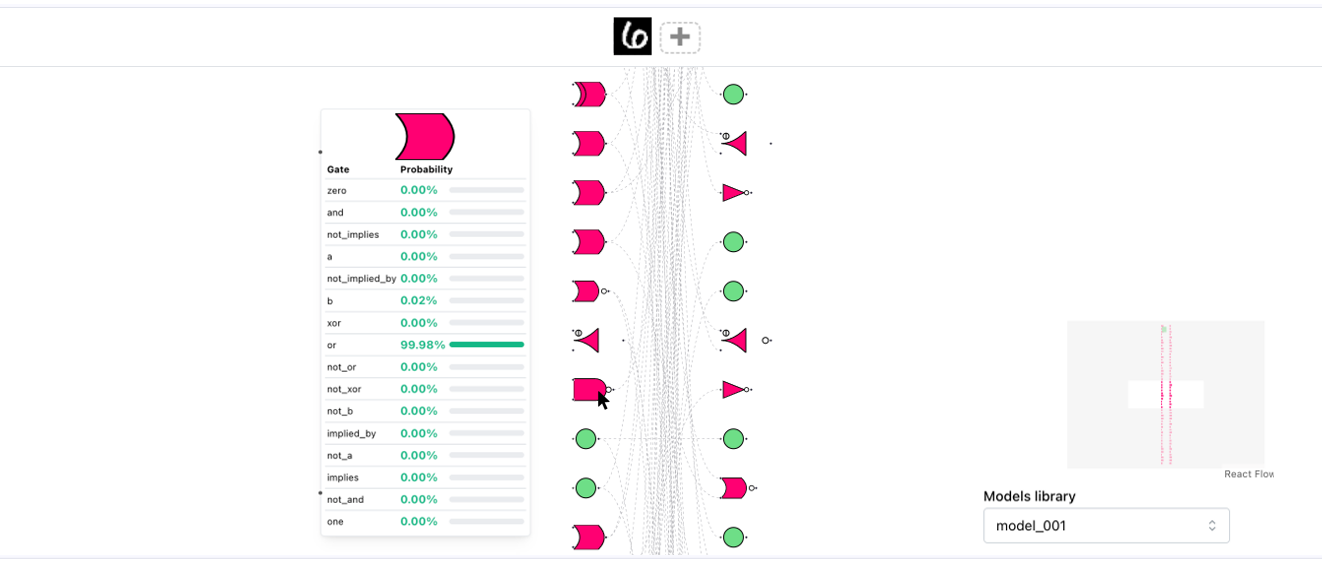
\includegraphics[width=0.934\linewidth]{Figures/difflogicvisualizer.png}}    
    \caption{Interface of DiffLogicVisualizer, demonstrating a network with 2 layers.}
    \label{fig:difflogic_figure}
\end{figure}